% открыть любую книгу по математике и улучшить шрифт в моем конспекте
\documentclass[12pt]{extarticle}

\usepackage{tikz}
\usepackage{graphicx}
\graphicspath{ {./pic/} }


%Russian-specific packages
%--------------------------------------
\usepackage[T2A]{fontenc}
\usepackage[utf8]{inputenc}
\usepackage[russian]{babel}
%--------------------------------------

%Hyphenation rules
%--------------------------------------
\usepackage{hyphenat}
\hyphenation{ма-те-ма-ти-ка вос-ста-нав-ли-вать}
%--------------------------------------

\setlength{\parindent}{0em} % space before par
\setlength{\parskip}{1em}   % spacing between pars

\usepackage{enumitem} % configure lists
% \setlist{noitemsep,topsep=0pt} % separation
\setlist{nosep} % separation
\setlist[itemize,1]{label=$\triangleleft$} % triangles looking to the left

% margin from paper borders
\usepackage[margin={0.8in, 0.3in}]{geometry}

\usepackage{amsmath}
\usepackage{amssymb}
\usepackage{amsfonts}
% 1 - Name
% 2 - Goes to the index
% 3 - Definition
% internal - some text about teorem
% \newenvironment{theorem}[3]{
% beginning
%     \vspace{0.5\parindent}
%     \par\index{#2}\emph{\underline{Th.} \textbf{#1} #3.}  % teorem's name
%     \par
% }{
% ending
    % \vspace{0.2\parindent}
% }

% 1 - Name
% 2 - Goes to index
% internal - Name's definition
\newenvironment{mydef}[2]{
% beginning
    \vspace{0.5\parindent}
    \par \index{#2} \emph{\underline{Def.} \textbf{#1}} -
}{
% ending
    \vspace{0.2\parindent}
}

% TODO
% \newcommand{hidefinition}

% 1 - Name
% 2 - Given
% 3 - Task
% internal - solution
\newenvironment{example}[3]{
    \vspace{0.5\parindent}
    \par\emph{\underline{Ex.}} #1
    \par \textbf{Given:} #2
    \par \textbf{Find:} #3
    \par \textbf{Solution:}
}{
    \vspace{0.5\parindent}
}

% displaystyle в каждом мас моде
\everymath{\displaystyle}

% vertical space for mathmode
\setlength{\abovedisplayskip}{0pt}
\setlength{\belowdisplayskip}{0pt}
\setlength{\abovedisplayshortskip}{0pt}
\setlength{\belowdisplayshortskip}{0pt}

% TODO: command for drawing box around text (so I can see why some artifact are

% TODO:
% \newcommand{grad}

% indent first line after section
\usepackage{indentfirst}

\usepackage{makeidx}
\makeindex

% keep this in the very bottom
% \usepackage[pdftex]{hyperref}
% remove red boxes around links
\usepackage[pdftex,pdfborderstyle={/S/U/W 0}]{hyperref} % this disables the boxes around links


\newcommand{\RE}{\mathrm{Re}\,}
\newcommand{\IM}{\mathrm{Im}\,}

\newcommand{\res}{\mathrm{res}\,}
\newcommand{\Ln}{\mathrm{Ln}\,}
\newcommand{\Arg}{\mathrm{Arg}\,}
\newcommand{\grad}{\mathrm{grad}\,}
\renewcommand{\v}{\upsilon}
\newcommand{\w}{\omega}
\renewcommand{\d}{\,d}

\begin{document}
\tableofcontents\newpage

\section{Комплексные числа и действия над ними.}
\textbf{Комплексным числом} называется выражение вида
\begin{displaymath}
x+iy
\end{displaymath}
где $x,\ y$ - действительные числа; $i$ - число, квадрат которого равен
минус единице.
\par \textit{Равные} числа:
\begin{displaymath}
    z_{1}=z_{2} \Leftrightarrow
        \left\{
            \begin{array}{ll}
                \RE\ z_{1} = \RE\ z_{2},\\
                \IM\ z_{1} = \IM\ z_{2}.
            \end{array}
        \right.
\end{displaymath}
\par \textit{Сопряженные} числа:
\begin{displaymath}
    \RE\ \bar{z} = \RE\ z,\ \ \IM\ \bar{z} = -\IM\ z
\end{displaymath}

\par
\begin{tabular}{l|c|c}
    \multicolumn{3}{c}{Действия над комплексными числами}\\\hline
    Действие & В алгебраической форме & В тригонометрической форме \\\hline
    Форма & $z=x+iy$ & $z=r(\cos \varphi + i\sin \varphi)$ \\
          & & $r=\sqrt{x^{2}+y^{2}},\ \tg{\varphi}=\frac{y}{x}$ \\\hline
    Сложение & $x=x_{1}+x_{2},\ y=y_{1}+y_{2} $ \\
    Вычитание & $x=x_{1}-x_{2},\ y=y_{1}-y_{2} $ \\

    Умножение & $x=x_{1}x_{2}-y_{1}y_{2},\ y=x_{1}y_{2}+x_{2}y_{1} $ &
    $r=r_{1}r_{2},\ \varphi=\varphi_{1}+\varphi_{2}$ \\

    Деление & Домножаем и делим на $\bar{z}$ &
    $r=\frac{r_{1}}{r_{2}},\ \varphi=\varphi_{1}-\varphi_{2}$ \\

    Возведение в степень &
    $\sum\limits_{k=0}^{n}C_{n}^{k}x^{n-k}(iy)^{k}$ &
    $r=r_{0}^{n},\ \varphi=n\varphi_{0}$\\

    Извлечение корня & $\RE{z}= \RE(x+iy)^{n},\ \IM{z}=\IM(x+iy)^{n}$ &
    $r=\sqrt[n]{r_{0}},\ \varphi_{k}=\frac{\varphi_{0}+2k\pi}{n},\ k=0..n-1$\\
    \hline
\end{tabular}
\begin{description}
    \item Доказательство умножения: втупую перемножаем и под скобками
        у тригонометрических функций окажется сложение $\varphi_{1}+\varphi_{2}$
    \item Доказательство извлечения корня: используем определение
        корня (комплексное число $z_{1}=\sqrt[n]{z}$ называется корнем
        $n$-й степени если $z=z_{1}^{n}$). Отсюда, по правилам умножения
        комплексных чисел получаем
        \begin{eqnarray*}
            \varphi_{k}=\frac{\varphi}{n}+\frac{2\pi k}{n}
        \end{eqnarray*}
\end{description}


\paragraph{Свойства операции комплексного сопряжения}
\begin{enumerate}
    \item $\overline{z_{1}\pm z_{2}}=\overline{z_{1}}\pm\overline{z_{2}}$
    \item $\overline{z_{1}\cdot z_{2}}=\overline{z_{1}}\cdot\overline{z_{2}}$
    \item $\overline{\left(\frac{z_{1}}{z_{2}}\right)}
        =\frac{\overline{z_{1}}}{\overline{z_{2}}}$
    \item $\overline{P_{n}(z)}=P_{n}(\overline{z})$
    \item $\overline{\left(\frac{P_{n}(z)}{Q_{m}(z)}\right)}
        =\frac{P_{n}(\overline{z})}{Q_{m}(\overline{z})}$
\end{enumerate}


\par \textbf{\textit{Формула Муавра}}
\begin{displaymath}
    (\cos\varphi+i\sin\varphi)^{n}=\cos n\varphi + i\sin n\varphi
\end{displaymath}

\paragraph{Бесконечно удаленная точка}\index{Бесконечно удаленная точка}
- определяется по тому же принципу что и с действительными числами.
Берем шар и из его верхней точки проводим хорду (делаем из нее луч,
который падает на плоскость). Чем короче хорда тем
дальше точка на плоскости.
\par Плоскость $\bar{C}=C\cup\left\{\infty\right\}$ -
\textit{расширенная комплексная плоскость}\index{Расширенная комплексная
плоскость}. Взаимно однозначное соответствие точек сферы и множества
$C$ называется \index{Стереографическая
проекция}\textit{стереографической проекцией}, сфера $S$ - \textit{сфера
Римана} \index{Сфера Римана}

\section{ФКП и действия над ними. Элементарные ФКП.}

\paragraph{Внутренняя точка.}\index{Внутренняя точка} Существует
$\varepsilon$-окрестность точки $z$, все точки которой принадлежат
множеству $E$
\paragraph{Область.}\index{Область} Множество $E$ называется область,
если: 1) каждая точка мн-ва $E$ - внутренняя точка этого мн-ва; 2) любые
две точки мн-ва $E$ можно соединить ломаной, все точки которой
принадлежат $E$
\paragraph{Замкнутая область}\index{Замкнутая область} - область +
граничные точки.
\paragraph{Односвязная область.}\index{Односвязная область} Любой контур
в области внутри себя содержит только область.
Внутренность любой Жордановой кривой, принадлежащей области, принадлежит области.
\paragraph{Многосвязная область.}\index{Многосвязная область} Область не
являющаяся односвязной.


\paragraph{Функция комплексной переменной.}\index{Функция комплексной
переменной} Говорят, что в области $D$ определена функция $w=f(z)$, если каждой
точке $z\in D$ поставлено в соответствие одно или несколько значений
$w$. (функция $w=f(z)$ осуществляет отображение точек из $z$ в точки
$w$).
\par Пусть $z=x+iy$ и $w=u+iv$. Тогда зависимость $w=f(z)$ между
комплексной фукнцией $w$ и комплексной переменной $z$ может быть описана
с помощью двух действительных функций $u$ и $v$ действительных
переменных $x$ и $y$:
\begin{displaymath}
    u=u(x,y),
    \ \ \ v=v(x,y).
\end{displaymath}

\par \textit{Элементарные} ФКП:
\paragraph{Формула Эйлера}\index{Формула Эйлера}
\begin{displaymath}
    e^{iz}=\cos z+i\sin z,
    \ \ e^{-iz}=\cos z-i\sin z,
\end{displaymath}
Доказательство: свойство функции
$e^{x}=\sum\limits_{n=0}^{\infty}\frac{x^{n}}{n!}$. Рассматриваем ряд
$\sum\limits_{n=0}^{\infty}\frac{z^{n}}{n!}$ и убеждаемся что он
абсолютно сходится при любом $z$. Поэтому можем ввести определение
\textit{показательной функции} $e^{z}$.
\par Рассматриваем разложение
$e^{ix}=\sum\limits_{n=0}^{\infty}\frac{i^{n}x^{n}}{n!}$.
Перегруппировываем получившиеся действительные и мнимые члены (там
окажется разложение синуса и косинуса относительно $x$), получаем
формулу Эйлера:
\begin{eqnarray*}
    e^{i\varphi}
    =\sum\limits_{k=0}^{\infty}\frac{(-1)^{k}x^{2k}}{(2k)!}
    +i\sum\limits_{k=1}^{\infty}\frac{(-1)^{k+1}x^{2k+1}}{(2k-1)!}
    =\cos{\varphi}+i\sin{\varphi}
\end{eqnarray*}
Свойства:
\begin{enumerate}
    \item Сложение по ф-ле Эйлера: $e^{z_{1}+z_{2}}=e^{z_{1}}\cdot e^{z_{2}}$
    \item \textbf{Периодичность.} $e^{z+2k\pi i}=e^{z}$
    \item Показательная функция не обращается в нуль ни при каком
        значении аргумента
    \item $|e^{z}|=e^{\RE{z}}$, $\arg{e^{z}}=\IM{z}$
\end{enumerate}

\par Логарифмическая функция $\Ln z$
\begin{eqnarray*}
    w=\Ln z=\ln{\left|z\right|}+i\Arg{z}
    =\ln{\left|z\right|}+i(\arg z+2k\pi)
\end{eqnarray*}
Доказательство: допустим $A=\ln{z}$, тогда $e^{z}=A$. Записываем
$A=u+iv$. Тогда получаем:
\begin{eqnarray*}
    e^{u+iv}=re^{i\varphi}
    \ \ \textmd{или}\ \ e^{u}\cdot e^{iv}=re^{i\varphi}
\end{eqnarray*}
из него получаем что
\begin{eqnarray*}
    &&u=\ln{r},\ (r>0);\\
    &&v=\varphi+2k\pi,\ k=0,\pm 1,\ldots
\end{eqnarray*}

\par Тригонометрические функции
\begin{eqnarray*}
    \cos z=\frac{e^{iz}+e^{-iz}}{2}
    ,\ \ \sin z=\frac{e^{iz}-e^{-iz}}{2i},\\
    \cos{y}=\frac{e^{iy}+e^{-iy}}{2}
    ,\ \ \sin{y}=\frac{e^{iy}-e^{-iy}}{2i}
\end{eqnarray*}

\par \textit{Гиперболические} функции:
\begin{eqnarray*}
    & \sh z=\frac{e^{z}-e^{-z}}{2},
    \ \ \ch z=\frac{e^{z}+e^{-z}}{2},\\
    & \textmd{th}\,z=\frac{\sh z}{\ch z},
    \ \ \cth z=\frac{\ch z}{\sh z}.
\end{eqnarray*}
$\cos{z},\ch{z}$ - четные, а остальные - нечетные. Более того:
\begin{eqnarray*}
    &&\cos{iz}=\ch{z},\ \ \ch{iz}=\cos{z}\\
    &&\sin{iz}=i\sh{z},\ \ \sh{iz}=i\sin{z}
\end{eqnarray*}
отсюда получаются такие формулы, как:
\begin{eqnarray*}
    \ch^{2}{z}-\sh^{2}{z}=1
    ,\ \ \ch^{2}{z}+\sh^{2}{z}=\ch{2z}
\end{eqnarray*}



Сравнивая формулы гиперболических функций и определения показательной
функции, видим, что:
\begin{eqnarray*}
    e^{iz}=\cos{z}+i\sin{z}\ \ e^{z}=\ch{z}+\sh{z}
\end{eqnarray*}


\section{Предел и непрерывность ФКП.}

Пусть дана последовательность $\left\{z_{n}\right\}$ комплексных чисел
\begin{displaymath}
    z_{1},z_{2},\ldots,z_{n},\ldots\ .
\end{displaymath}
\paragraph{Предел последовательности}\index{Предел последовательности} - 
комплексное число $a$, если для любого положительного числа
$\varepsilon$ можно указать такой номер $N=N(\varepsilon)$, начиная
с которого все элементы $z_{n}$ этой последовательности
удовлетворяют неравенству
\begin{displaymath}
    \left|z_{n}-a\right|<\varepsilon
    \ \textmd{при} \ n\geqslant N(\varepsilon).
\end{displaymath}

\par \textbf{Теорема 1.} Последовательность
$\left\{z_{n}=x_{n}+y_{n}\right\}$ сходится к числу $a=\alpha+i\beta$
тогда и только тогда, когда
\begin{displaymath}
    \lim\limits_{n\rightarrow \infty}x_{n}=\alpha,
    \ \ \ \lim\limits_{n\rightarrow \infty}y_{n}=\beta
\end{displaymath}
\par \textit{Доказательство:} Допустим последовательность
$\left\{z_{n}\right\}$ сходится, тогда беря в рассмотрение:
\begin{eqnarray*}
    |a_{n}-a|\leqslant |z_{n}-z| < \varepsilon
    \ \ \textmd{и}
    \ \ |b_{n}-b|\leqslant |z_{n}-z| < \varepsilon
\end{eqnarray*}
можем сказать что сходятся соответственно $\left\{a_{n}\right\}$ и
$\left\{b_{n}\right\}$. В обратную сторону:
\begin{eqnarray*}
    |z_{n}-z|=\sqrt{(a_{n}-a)^{2}+(b_{n}-b)^{2}}
\end{eqnarray*}

\par \textbf{Теорема 2.} Всякая сходящаяся последовательность
ограничена.

\par Свойства сх-ся последовательностей комплексных чисел:
\begin{enumerate}
    \item $\lim\limits_{n\rightarrow \infty}(z_{n}\pm\tau_{n})=a\pm b;$
    \item $\lim\limits_{n\rightarrow \infty}(z_{n}\tau_{n})=ab;$
    \item $\lim\limits_{n\rightarrow \infty}\frac{z_{n}}{\tau_{n}}
        =\frac{a}{b}\ (\tau_{n}\neq0,\ b\neq0).$
\end{enumerate}

\paragraph{Окрестность бесконечно удаленной точки}
\index{Окрестность бесконечно удаленной точки} - 
совокупность точек $z$, удовлетворяющих неравенству
$\left|z\right|>R$ (с присоединением бесконечно удаленной точки).

\paragraph{Окрестность точки $z_{0}$}\index{Окрестность точки} -
всякая область, содержащая эту точку.

\paragraph{$\varepsilon$-окрестность $z_{0}$}
\index{$\varepsilon$-окрестность} -
мн-во всех точек $z$, удовлетворяющих
неравенству $\left|z-z_{0}\right|<\varepsilon$

\paragraph{Предел функции $f(z)$ в точке $z_{0}$} -
\index{Предел функции в точке}
число $A$, если для любого числа $\varepsilon>0$ можно указать такое
число $\delta=\delta(\varepsilon)>0$, что для всех точек
$z\in\Omega$, удовлетворяющих условию
$0<\left|z-z_{0}\right|<\delta$ выполняется неравенство
\begin{displaymath}
    \left|f(z)-A\right|<\varepsilon
\end{displaymath}
В этом случае пишут
\begin{displaymath}
    \lim\limits_{z\rightarrow z_{0}}f(z)=A.
\end{displaymath}
Еще одно определение. Если для любой последовательности
$\left\{z_{n}\right\},\ z_{n}\neq z_{0}$, сходящейся к точке
$z_{0}$, соответствующая ей последовательность значений функции
$\left\{f(z_{n})\right\}$ сходится к одному и тому же комплексному
числу $A$.
\par Из первого вытекает второе: берем $\varepsilon$, выбираем для него
$\delta$, находим для него $N[\delta(\varepsilon)]$, и так как
$|f(z_{n})-A|<\varepsilon$ то в силу произвольности выбора $\varepsilon$
функция $f(z)$ удовлетворяет и второму определению
\par В обратную сторону: предположим что не выполняется. Тогда можно
указать такое $\varepsilon_{0}>0$, что для любого $\delta_{n}>0$
найдется такая точна $z_{n}\in E$, что при $0 <
|z_{n}-z_{0}|<\delta_{n}$ будет выполнено неравенство
$|f(z_{n})-|>\varepsilon_{0}$. Выберем
последовательность$\left\{\delta_{n}\right\} \to 0$ и соответствующую
последовательность $\left\{z_{n}\right\}$ из поставленных условий
очевидно что $\left\{f(z_{n})\right\}$ не сходится к $A$. Но полученный
результат противоречит определению.

\paragraph{Непрерывность в точке $z_{0}\in D$} -
\index{Непрерывность в точке}
если выполняется равенство
\begin{displaymath}
    \lim\limits_{z\rightarrow z_{0}}f(z)=f(z_{0})
\end{displaymath}

\section{Дифференцируемость ФКП. Условия Коши-Римана.}

Пусть дана функция $w=f(z)$ определена в некоторой области $D$
комплексного переменного $z$. Пусть точки $z$ и $z+\Delta z$ принадлежат
области $D$. Обозначим
\begin{displaymath}
    \Delta w=f(z+\Delta z)-f(z),
    \ \ \ \Delta z=\Delta x+i\Delta y
\end{displaymath}

\paragraph{Дифференцируемость в точке $z\in D$} -
\index{Дифференцируемость в точке}
соотношение $\frac{\Delta w}{\Delta z}$ имеет конечный предел при
$\Delta z \to 0$. Этот предел называется \textit{производной} ф-ции
$f(z)$ в данной точке $z$.
\begin{displaymath}
    w'=f'(z)=\lim\limits_{\Delta z\rightarrow 0}\frac{\Delta
    w}{\Delta z}.
\end{displaymath}
\par Если $z=x+iy$, $w=f(z)=u(x,y)+iv(x,y)$, то в каждой точке
дифференцируемости функции $f(z)$ существуют частные производные и
выполняются соотношения
\begin{displaymath}
\frac{\partial u}{\partial x}=\frac{\partial v}{\partial y},
\ \ \frac{\partial u}{\partial y}=-\frac{\partial v}{\partial x};
\end{displaymath}
- \textbf{\textit{условия Коши-Римана}}\index{Условия Коши-Римана}. Доказательство:
\textit{Из существования предела комплексного выражения следует
существование пределов его действительной и мнимой частей.} Положим $\Delta
z=\Delta x$. Получаем выражение:
\begin{eqnarray*}
    &&f'(z_{0})=\\
    &&=\lim\limits_{\Delta x\rightarrow 0}\frac{u(x_{0}+\Delta
    x,y_{0})-u(x_{0},y_{0})}{\Delta x}
    +i\lim\limits_{\Delta x\rightarrow 0}\frac{v(x_{0}+\Delta
    x,y_{0})-v(x_{0},y_{0})}{\Delta x}=\\
    &&=u_{x}(x_{0},y_{0})+iv_{x}(x_{0},y_{0})
\end{eqnarray*}
положим $\Delta z=i\Delta y$, получаем:
\begin{eqnarray*}
&&f'(z_{0})=\\
&&=-i\lim\limits_{\Delta y\rightarrow 0}
\frac{u(x_{0},y_{0}+\Delta y)-u(x_{0},y_{0})}{\Delta y}
+\lim\limits_{\Delta y\rightarrow 0}
\frac{v(x_{0},y_{0}+\Delta y)-v(x_{0},y_{0})}{\Delta y}=\\
&&=-iu_{y}(x_{0},y_{0})+v_{y}(x_{0},y_{0})
\end{eqnarray*}
\par В обратную сторону: приращения $u$ и $v$ могут быть записаны в
виде:
\begin{eqnarray*}
    u(x_{0}+\Delta x,y_{0}+\Delta y)-u(x_{0},y_{0})
    =u_{x}(x_{0},y_{0})\Delta x+u_{y}(x_{0},y_{0})\Delta y+\xi(x,y)\\
    v(x_{0}+\Delta x,y_{0}+\Delta y)-v(x_{0},y_{0})
    =v_{x}(x_{0},y_{0})\Delta x+v_{y}(x_{0},y_{0})\Delta y+\eta(x,y)
\end{eqnarray*}
преобразуем его к виду (исп. Коши-Римана):
\begin{eqnarray*}
& \frac{f(z_{0}+\Delta z)-f(z_{0})}{\Delta z} &
=u_{x}(x_{0},y_{0})\frac{\Delta x+i\Delta y}{\Delta x+i\Delta y}
+v_{x}(x_{0},y_{0})\frac{i\Delta x -\Delta y}{\Delta x+i\Delta y}+\\
&&\frac{\xi(x,y)+i\eta(x,y)}{\Delta x+i\Delta y}
=u_{x}(x_{0},y_{0})+iv_{x}(x_{0},y_{0})+\frac{\zeta(z)}{\Delta zx}\\
&&(\zeta(z)=\xi(x,y)+i\eta(x,y))
\end{eqnarray*}

\paragraph{Геометрический смысл производной.}
\index{Геометрический смысл производной}
Предположим, что $f'(z_{0})\neq 0$:
\begin{eqnarray*}
    f'(z_{0})=\lim\limits_{\Delta z\rightarrow 0}
    \frac{\Delta w}{\Delta z}=ke^{i\alpha}
\end{eqnarray*}
выберем такой способ стремления $\Delta z$ к нулю, при котором точки
$z=z_{0}+\Delta z$ лежат на кривой $\gamma_{1}$. Очевидно,
соответствующие им точки $w=w_{0}+\Delta w$ лежат на кривой
$\Gamma_{1}$. Из формулы выше следует, что:
\begin{eqnarray*}
    \alpha=\arg f'(z_{0})=\lim\limits_{\Delta z\rightarrow 0}\arg\Delta
    w-\lim\limits_{\Delta z\rightarrow 0}\arg\Delta
    z=\Phi_{1}-\varphi_{1}
\end{eqnarray*}
то есть $\alpha$ имеет смысл угла $\Phi_{1}$ вектора касательной к
кривой $\Gamma_{1}$ в точке $w_{0}$ (аналогично для $\gamma_{1}$). Более
того, отсюда следует, что \textit{при отображении осуществляемом
аналитической функцией $f(z)$, удовлетворяющей условию $f'(z_{0})\neq
0$, угол $\varphi=\varphi_{2}-\varphi_{1}$ между любыми кривыми
$\gamma_{2},\gamma_{1}$, пересекающимися в точке $z_{0}$, равен углу
$\Phi=\Phi_{2}-\Phi_{1}$, между их образами в точке $w_{0}=f(z_{0})$.
Сохраняется не только абсолютная величина углов, но и направление углов
- свойство сохранения углов}\index{Свойство сохранения углов}
\par Аналогично из первого соотношения получим:
\begin{eqnarray*}
    k=|f'(z_{0})|=\lim\limits_{\Delta z\rightarrow 0}\frac{|\Delta
    w|}{|\Delta z|}
\end{eqnarray*}
то есть с точностью до величин более высокого порядка малости имеет
место равенство $|\Delta w|=k|\Delta z|$. Геометрический смысл:
\textit{при отображении, осуществляемом аналитической функцией,
удовлетворяющей условию $f'(z_{0})\neq 0$, бесконечно малые линейные
элементы преобразуются подобным образом, причем $|f'(z_{0})|$ определяет
коэффициент преобразования подобия. Это свойство - свойство поятоянства
растяжения}\index{Свойство постоянства растяжения}

\paragraph{Конформное отображение.} \index{Конформное отображение}
Отображение окрестности точки $z_{0}$ на окрестность точки $w_{0}$,
осуществляемое аналитической функцией $w=f(z)$ и обладающее в точке
$z_{0}$ свойством сохранения углов и постоянством растяжений, называется
конформным отображением.

\paragraph{Аналитическая функция в точке $z\in D$} -
\index{Аналитическая функция в точке}
функция дифференцируема как в самой точке, так и в некоторой ее
окрестности. Функция $f(z)$ называется аналитической \textit{в
области} $D$, если она дифференцируема в каждой точке этой области.
Для любой аналитической функции $f(z)$ имеем:
\begin{displaymath}
    f'(z)
    =\frac{\partial u}{\partial x}+i\frac{\partial v}{\partial x}
    =\frac{\partial v}{\partial y}-i\frac{\partial u}{\partial y}
    =\frac{\partial u}{\partial x}-i\frac{\partial u}{\partial y}
    =\frac{\partial v}{\partial y}+i\frac{\partial v}{\partial x}
\end{displaymath}
\textit{производную берем как у вещественной, но частные производные
связаны уравнениями}
\par Свойства:
\begin{enumerate}
    \item Если ф-ция $f(z)$ является наалитической в области $G$, то она
        непрерывна в этой области
    \item $f_{1}(z),f_{2}(z)$ - аналитические функции в области $G$, их
        сумма, произведение - также аналитические функции в области $G$
        ($\frac{f_{1}(z)}{f_{2}(z)}$ аналитическая там, где
        $f_{2}(z)\neq 0$)
    \item Последовательное применение двух аналитических функций -
        аналитическая функция
    \item Обратная к аналитической функции - тоже аналитическая фукнция,
        причем $f'(z_{0})=\frac{1}{\varphi'(\omega_{0})}$
        \subitem Доказательство: Для существовани обратной функции
        необходимо, чтобы уравнения $u=u(x,y)$ и
        $\upsilon=\upsilon(x,y)$ можно было разрешить относительно $x,y$
        в окрестности точки $\omega_{0}$. Для этого достаточно, чтобы в
        окрестности точки $z_{0}$ выполнялось условие
        \begin{eqnarray*}
            \left|\begin{array}{cc}
                u_{x} & u_{y} \\ \upsilon_{x} & \upsilon_{y}
            \end{array} \right| =
            u_{x}\upsilon_{y}-u_{y}\upsilon_{x}\neq 0
        \end{eqnarray*}
        Из уравнения
        \begin{eqnarray*}
        \frac{\Delta z}{\Delta \omega}=\frac{1}{\frac{\Delta
        \omega}{\Delta z}}
        \end{eqnarray*}
        легко доказать существование и непрерывность производной
        $\varphi'(\omega_{0})$ ($|f'(z_{0})\neq 0$)
    \item Пусть задана функция $u(x,y)$ являющаяся действительной частью
        аналитической функции $f(z)$. Тогда мнимая часть этой функции
        определяется с точностью до аддитивной постоянной.
        \begin{eqnarray*}
            \d\v=\v_{x}\d{x}+\v_{y}\d{y}
            =-u_{y}\d{x}+u_{x}\d{y}
        \end{eqnarray*}
    \item $u(x,y)=C$ и $\v(x,y)=C$ взаимно ортогональны
        ($\grad{u}\cdot\grad{\v}=0$ градиент ортогонален линии уровня)
\end{enumerate}


\section{Интегральная формула Коши.}
Функция $f(z)$ - аналитическая в области $D$, ограниченная
кусочно-гладким замкнутым контуром $C$ (и на самом контуре), то
справедлива \textit{интегральная формула Коши}:
\begin{displaymath}
    f(z_{0})=\frac{1}{2\pi i}\int\limits_{C}\frac{f(z)dz}{z-z_{0}},
    \ \ (z_{0}\in D)
\end{displaymath}
контур $C$ обходится так, что область $D$ остается все время слева.

\paragraph{Вывод формулы Коши}
Пусть $f(z)$ аналитична в $D$, ограниченной контуром $C$. Возьмем
произвольную внутреннюю точку $z_{0}$ и построим замкнутый контур
$\Gamma$ (целиком лежит в области $D$ и содержит $z_{0}$). Рассмотрим
вспомогательную функцию:
\begin{eqnarray*}
    \varphi(z)=\frac{f(z)}{z-z_{0}}
\end{eqnarray*}
очевидно является аналитической в области $D$ за исключением т. $z_{0}$.
Поэтому если мы в области $D$ окружим эту точку контуром $\gamma$
(лежащим внутри $\Gamma$), то ф-ция $\varphi(z)$ будет аналитической в
двухсвязной области $D^{*}$, заключенной между контурами $\Gamma$ и
$\gamma$. Согласно теореме Коши:
\begin{eqnarray*}
    \int\limits_{\Gamma^{+}}\frac{f(\zeta)}{\zeta-z_{0}}\d{\zeta}
    +\int\limits_{\gamma^{-}}\frac{f(\zeta)}{\zeta-z_{0}}\d{\zeta}
    =0
\end{eqnarray*}
Изменив направление интегрирования во втором интеграле, получим:
\begin{eqnarray*}
    \int\limits_{\Gamma^{+}}\frac{f(\zeta)}{\zeta-z_{0}}\d{\zeta}
    =\int\limits_{\gamma^{+}}\frac{f(\zeta)}{\zeta-z_{0}}\d{\zeta}
\end{eqnarray*}
Интегралы по обе стороны не зависят от выбранного контура. Для
дальнейших рассмотрений возьмем в качестве контура $\gamma$ окружность
$\gamma_{\rho}$ (круг радиусом $\rho$ с центром в точке $z_{0}$).
Положив $\zeta=z_{0}+\rho e^{i\varphi}$:
\begin{eqnarray*}
    \int\limits_{\Gamma^{+}}\frac{f(\zeta)}{\zeta-z_{0}}\d{\zeta}
    =i\int\limits_{0}^{2\pi}f(\zeta)\d{\varphi}
\end{eqnarray*}
Раскроем правую часть таким образом
\begin{eqnarray*}
    \int\limits_{0}^{2\pi}f(\zeta)\d{\varphi}
    =\int\limits_{0}^{2\pi}[f(\zeta)-f(z_{0})]\d{\varphi}
    +\int\limits_{0}^{2\pi}f(z_{0})\d{\varphi}
    =\int\limits_{0}^{2\pi}[f(\zeta)-f(z_{0})]\d{\varphi}+2\pi f(z_{0})
\end{eqnarray*}
Устремив $\rho$ к нулю. Получаем из определения непрерывности что для
любого $\varepsilon$ можно указать такое $\rho$ что
$|f(\zeta)-f(z_{0})|<\varepsilon$ для $|\zeta-z_{0}|<\rho$. Отсюда, при
$\rho\to 0$ существует предел
\begin{eqnarray*}
    \lim\limits_{\rho\rightarrow
    0}\int\limits_{0}^{2\pi}[f(\zeta)-f(z_{0})]\d{\varphi}=0
\end{eqnarray*}
Получаем что
\begin{eqnarray*}
    \int\limits_{\gamma^{+}}\frac{f(\zeta)}{\zeta-z_{0}}\d{\zeta}
    =2\pi if(z_{0})
\end{eqnarray*}
и согласно исходному уравнению
\begin{eqnarray*}
    f(z_{0})=\frac{1}{2\pi
    i}\int\limits_{\Gamma}\frac{f(\zeta)}{\zeta-z_{0}}\d{\zeta}
\end{eqnarray*}

\paragraph{Советы по решению}
\par Случай когда внутри области \textit{больше одной особой точки}:
\begin{enumerate}
    \itemsep0em
    \item Разложи дробь на несколько дробей
    \item Выделяем непересекающиеся области вокруг особых точек, и
        получаем что значение общего интеграла является суммой
        интегралов от этих самых маленьких областей
\end{enumerate}

\par Просто полезная формула для вычислений:
\begin{eqnarray*}
    f^{(n)}(z_{0})=\frac{n!}{2\pi i}\int\limits_{\Gamma}
    \frac{f(z)}{(z-z_{0})^{n+1}}dz
\end{eqnarray*}


\section{Аналитические и гармонические ряды.}

\paragraph{Коэффициенты степенного ряда}\index{Коэффициенты степенного ряда}
выражаются через значения суммы ряда $f(z)$ и ее производных в цетре
круга сходимости по формулам:
\begin{eqnarray*}
    c_{n}=\frac{1}{n!}f^{(n)}(z_{0})
\end{eqnarray*}

\paragraph{Радиус сходимости}
\index{Радиус сходимости} ряда $\sum\limits_{n=0}^{\infty}c_{n}z^{n}$:
\begin{displaymath}
    R=\overline{\lim\limits_{n\rightarrow
    \infty}}\frac{|c_{n}|}{\left|c^{n+1}\right|},\ \ c_{n}\neq 0
\end{displaymath}
или
\begin{displaymath}
    R=\overline{\lim\limits_{n\rightarrow \infty}}\frac{1}{\sqrt[n]{\left|c_{n}\right|}}
\end{displaymath}
При доказательстве, мы мажорируем одну последовательность и показываем
что она сходится. Вторую наоборот - показываем что расходится.

\paragraph{Теорема Абеля.}\index{Теорема Абеля} Если степенной ряд
$\sum\limits_{n=0}^{\infty}c_{n}(z-z_{0})^{n}$ сходится в некоторой
точке $z_{1}\neq z_{0}$, то он абсолютно сходится и в любой точке $z$,
удовлетворяющей условию $|z-z_{0}|<|z_{1}-z_{0}|$; причем в круге
$|z_{1}-z_{0}|\leqslant\rho$, меньшего $|z_{1}-z_{0}|$, ряд сходится
равномерно

\paragraph{Теорема Тейлора.}\index{Теорема Тейлора} Функция $f(z)$
аналитическая внутри круга $|z-z_{0}|<R$, может быть представлена в этом
круге сходящимся степенным рядом
$f(z)=\sum\limits_{n=0}^{\infty}c_{n}(z-z_{0})^{n}$, причем этот ряд
определен однозначно.


\section{Оценки коэффициентов ряда Тейлора.}
\paragraph{Теорема Тейлора.}\index{Теорема Тейлора} Функция $f(z)$,
аналитическая внутри круга $|z-z_{0}|<R$, может быть представлена в этом
круге сходящимся степенным рядом
$f(z)=\sum\limits_{n=0}^{\infty}c_{n}(z-z_{0})^{n}$, причем этот ряд
определен однозначно
\par Док-во: Выберем произвольную точку $z$ внутри круга $|z-z_{0}|<R$ и построим
окружность $C_{\rho}$ с центром в точке $z_{0}$ радиуса $\rho < R$
содержащую точку $z$ внутри. Т.к. функция в этой области аналитическая,
по формуле Коши имеем:
\begin{eqnarray*}
    f(z)=\frac{1}{2\pi
    i}\int\limits_{C_{\rho}}\frac{f(\zeta)}{\zeta-z}\d{\zeta}
\end{eqnarray*}
Осуществим в подынтегральном выражении преобразование
\begin{eqnarray*}
\frac{1}{\zeta-z}
=\frac{1}{\zeta-z_{0}}\frac{1}{1-\frac{z-z_{0}}{\zeta-z_{0}}}
=\frac{1}{\zeta-z_{0}}\sum\limits_{n=0}^{\infty}\frac{(z-z_{0})^{n}}{(\zeta-z_{0})^{n}}
\end{eqnarray*}
При $\zeta\in C_{\rho}$ ряд сходится равномерно по $\zeta$, т.к. он
мажорируется сходящимся числовым рядом
$\sum\limits_{n=0}^{\infty}\frac{|z-z_{0}|^{n}}{\rho^{n+1}}$
\par Совмещая последние два уравнения, получаем:
\begin{eqnarray*}
    f(z)=\sum\limits_{n=0}^{\infty}\frac{1}{2\pi i}
    \int\limits_{C_{\rho}}\frac{f(\zeta)\d{\zeta}}{(\zeta-z_{0})^{n+1}}(z-z_{0})^{n}
\end{eqnarray*}
Введя обозначение:
\begin{eqnarray*}
    c_{n}=\frac{1}{2\pi i}\int\limits_{C_{\rho}}
    \frac{f(\zeta)}{(\zeta-z_{0})^{n+1}}\d{\zeta}
    =\frac{f^{(n)}(z_{0})}{n!}
\end{eqnarray*}
перепишем в виде сходящегося в выбранной точке $z$ степенного ряда
\begin{eqnarray*}
    f(z)=\sum\limits_{n=0}^{\infty}c_{n}(z-z_{0})^{n}
\end{eqnarray*}
\par Доказательство единственности: допустим есть другое сходящееся
разложение в указанном круге, на основании формулы для коэффициентов
$c'_{n}=\frac{f^{(n)}(z_{0})}{n!}$ получим те же самые коэффициенты что
и были.

\section{Интеграл ФКП. Его свойства и вычисление.}
\subsection{Определение}
\begin{eqnarray*}
    S(\zeta_{i},\zeta_{i}^{*})=\sum\limits_{i=1}^{n}f(\zeta_{i}^{*})\Delta\zeta_{i}
\end{eqnarray*}
где $\zeta_{i}^{*}$ - произвольная точка $i$-й частичной дуги. Если при
$\max |\Delta\zeta_{i}|\to 0$ существует предел сумм, не зависящий ни от
способа разбиения кривой $C$ ни от выбора точек $\zeta_{i}^{*}$, то этот
предел называется интегралом от функции $f(\zeta)$ по кривой $C$ и
обозначается как
\begin{eqnarray*}
    \int\limits_{C}f(\zeta)\d{\zeta}
\end{eqnarray*}


\subsection{Свойства}
Если принять $f(\zeta_{i}^{*})=u(P_{i}^{*})+i\v(P_{i}^{*})$,
$\Delta\zeta_{i}=\Delta\xi_{i}+i\Delta\eta_{i}$, где
$P_{i}(\xi_{i}^{*},\eta_{i}^{*})$ - точка кривой $C$ на плоскости $xy$,
можем представить интеграл в виде
\begin{eqnarray*}
    \int\limits_{C}f(\zeta)\d{\zeta}
    =\int\limits_{C}u\d{\xi}-\v\d{\eta}
    +i\int\limits_{C}u\d{\eta}-\v\d{\xi}
\end{eqnarray*}

Если $f(z)$- аналитическая функция в односвязной области $D$, то
интеграл не зависит от пути интегрирования
\begin{displaymath}
    \int\limits_{L}f(z)dz = 0
\end{displaymath}

\begin{enumerate}
    \item
        $\int\limits_{AB}f(\zeta)\d{\zeta}=-\int\limits_{BA}f(\zeta)\d{\zeta}$
    \item
        $\int\limits_{C_{1}}f(\zeta)\d{\zeta}+\int\limits_{C_{2}}f(\zeta)\d{\zeta}
        =\int\limits_{C_{1}+C_{2}}f(\zeta)\d{\zeta}$
    \item Если $a$ - комплексная постоянная, то:
        \begin{eqnarray*}
            \int\limits_{C}af(\zeta)\d{\zeta}=a\int\limits_{C}f(\zeta)\d{\zeta}
        \end{eqnarray*}
    \item
        $\int\limits_{C}\left\{f_{1}(\zeta)+f_{2}(\zeta)\right\}\d{\zeta}
        =\int\limits_{C}f_{1}(\zeta)\d{\zeta}+\int\limits_{C}f_{2}(\zeta)\d{\zeta}$
    \item $\left|\int\limits_{C}f(\zeta)\d{\zeta}\right|
        \leqslant \int\limits_{C}\left|f(\zeta)\right|\d{s}$, $\d{s}$ -
        дифференциал длины дуги кривой $C$
    \item
        $\int\limits_{C}f(z)\d{z}=\int\limits_{\Gamma}f[\varphi(\zeta)]\varphi'(\zeta)\d{\zeta}$,
        где $z=\varphi(\zeta)$ - аналитическая функция $\zeta$,
        устанавливающая взаимно-однозначное соответствие между кривыми
        $C$ и $\Gamma$
\end{enumerate}

\subsection{Вычисление. To write}
\par Путь интегрирования полупрямая или окружность? Замена:
\begin{displaymath}
    z-z_{0}=\rho e^{i\varphi}
\end{displaymath}
\par Пусть однозначная функция $f(z)$ определена и непрерывна в области $D$,
а $C$ - кусочно-гладкая замкнутая или незамкнутая ориентированная
кривая, лежащая в $D$. Пусть $z=x+iy$, $f(z)=u+iv$, где $u=u(x,y)$,
$v=v(x,y)$. Тогда:
\begin{displaymath}
    \int\limits_{C}f(z)dz=\int\limits_{C}udx-vdy +
    i\int\limits_{C}vdx+udy
\end{displaymath}


\section{Основная теорема Коши для односвязной области.}

\par Либо это (Теорема Коши). Пусть в односвязной области $D$ задана
однозначная аналитическая функция $f(z)$. Тогда интеграл от этой функции
по любому замкнутому контуру $\Gamma$, целиком лежащему в области $D$
равен нулю
\par Доказательство:
\begin{eqnarray*}
    \int\limits_{\Gamma}f(\zeta)\d{\zeta}=\int\limits_{\Gamma}u\d{x}-\v\d{y}
    +i\int\limits_{\Gamma}u\d{y}+\v\d{x}
\end{eqnarray*}
Дальше воспользуемся формулой
\begin{eqnarray*}
    \int\limits_{C}P\d{x}+Q\d{y}
    =\iint\limits_{D}\left\{\frac{\partial Q}{\partial x}
    -\frac{\partial P}{\partial y}\right\}\d{x}\d{y}
\end{eqnarray*}
которая требует чтобы функции $P,Q$ были непрерывны в замкнутой области
$\overline{D}$, ограниченной кусочно гладким контуром $C$, а их частные
производные первого порядка непрерывны в $D$. Добавив к этому условие
Коши-Римана получаем что интеграл будет равен нулю.

\paragraph{Теорема о составном интеграле.} Если область многосвязная,
то имеет место \index{Теорема о составном интеграле}:
Пусть $f(z)$ является аналитической функцией в многосвязной области $D$,
ограниченной извне контуром $C_{0}$, а изнутри контурами
$C_{1},C_{2},\ldots,C_{n}$ и пусть $f(z)$ непрерывна в замкнутой области
$\bar{D}$. Тогда $\int\limits_{C}f(\zeta)\d\zeta=0$, где $C$ - полная
граница области $D$, причем обход границы $C$ происходит в положительном
направлении.
\begin{eqnarray*}
    \int\limits_{C_{0}^{+}}f(\zeta)\d{\zeta}
    +\int\limits_{C_{1}^{-}}f(\zeta)\d{\zeta}
    +\ldots
    +\int\limits_{C_{n}^{-}}f(\zeta)\d{\zeta}
    =0
\end{eqnarray*}
Док-во: проводим гладкие кривые $\gamma_{1},\ldots,\gamma_{n}$,
соединяющие контур $C_{0}$ с контурами $C_{1},C_{2},\ldots$. Тогда
область будет односвязной и интеграл по границе равен нулю. Но интегралы
по $\gamma_{i}$ проходятся дважды в противоположных направлениях и при
суммировании выпадают.


\section{Вычеты. Основная теорема о вычетах. Вычисление вычетов.}
\subsection{Вычеты}

\paragraph{Вычет функции $f(z)$ в точке $z_{0}$}
\index{Вычет}
обозначается символом $\res f(z_{0})$ и определяется равенством
\begin{displaymath}
    \res f(z_{0})=\frac{1}{2\pi i}\oint\limits_{\gamma}f(z)dz
\end{displaymath}
где $z_{0}$ - изолированная особая точка функции $f(z)$, $\gamma$ -
контур полностью лежащий в области аналитичности функции и содержащий
единственную особую точку $z_{0}$ ф-ции $f(z)$. Другие
обозначения: $\res[f(z),z_{0}]$, $\res_{z=z_{0}}f(z)$
\par Вычет равен коэффициенту при минус первой степени в лорановском
разложении $f(z)$ в окрестности точки $z_{0}$
\begin{displaymath}
    \res f(z_{0})=c_{-1}
\end{displaymath}

\subsection{Основная теорема о вычетах}\label{основная теорема о вычетах}
\textit{Основная теорема теории вычетов.}
Функция $f(z)$ является аналитической на границе $C$ области $D$ и всюду
внутри области, за исключением конечного числа особых точек
$z_{1},z_{2},\ldots,z_{n}$, то
\begin{displaymath}
    \int\limits_{C}f(z)dz=2\pi i\sum\limits_{k=1}^{n}\res f(z_{k})
\end{displaymath}
\par Доказательство: Выделим каждую из особых точек $z_{k}$ функции
$f(z)$ замкнутым контуром $\gamma_{k}$, не содержащим внутри других
особых точек, кроме точки $z_{k}$. В построенной многосвязной области
функция $f(z)$ всюду аналитична. Отсюда, по второй теореме Коши получим:
\begin{eqnarray*}
    \int\limits_{\Gamma^{+}}f(\zeta)\d\zeta
    +\sum\limits_{k=1}^{N}\int\limits_{\gamma_{k}^{-}}f(\zeta)\d\zeta
    =0
\end{eqnarray*}
Перенеся второе слагаемое вправо, в силу определения вычета получим:
\begin{eqnarray*}
    \int\limits_{\Gamma^{+}}f(\zeta)\d\zeta
    =2\pi i\sum\limits_{k=1}^{N}\res[f(z),z_{k}]
\end{eqnarray*}




\subsection{Вычисление вычетов}

\begin{itemize}
    \itemsep0em
    \item Устранимая особая точка
        \subitem $\res f(z_{0}) = 0$
    \item Полюс $n$-го порядка
        \subitem $\res
        f(z_{0})=\frac{1}{(n-1)!}\lim\limits_{z\rightarrow
        z_{0}}\frac{d^{n-1}}{dz^{n-1}}\left\{f(z)(z-z_{0})^{n}\right\}$
    \item Если функция $f(z)$ в окрестности точки $z_{0}$ представима
        как частное двух аналитических функций
        \begin{displaymath}
            f(z)=\frac{\varphi(z)}{\psi(z)}
        \end{displaymath}
        причем $\varphi(z_{0})\neq 0$, $\psi(z_{0})=0$, а
        $\psi'(z_{0})\neq 0$, т.е. $z_{0}$ - простой полюс функции
        $f(z)$, то
        \begin{displaymath}
            \res f(z_{0})=\frac{\varphi(z_{0})}{\psi'(z_{0})}
        \end{displaymath}
    \item Существенно особая точка - вручную находишь коэффициент $c_{-1}$
\end{itemize}

Если функция $f(z)$ имеет вид $f(z)=\frac{\varphi(z)}{\psi(z)}$, где
аналитические функции $\varphi(z)$ и $\psi(z)$ имекют нули выше первого
порядка, можно замить их разложениями в ряд Тейлора в окреестности точки
$z_{0}$

\subsection{Вычет функции относительно бесконечно удаленной точки}
\paragraph{Функция $f(z)$ аналитична в бесконечно удаленной точке}
\index{Аналитичность в бесконечно удаленной точке}
если функция
\begin{displaymath}
    \varphi(\zeta)=f\left(\frac{1}{\zeta}\right)
\end{displaymath}
аналитична в точке $\zeta=0$
\par Тип точки зависит от конечности, бесконечности или существования
$\lim\limits_{z\rightarrow \infty}f(z)$. Чтобы понять это, выполняешь
следующие действия: $\zeta=\frac{1}{z}$, затем рассматриваешь тип точки
в функции $f\left(\frac{1}{\zeta}\right)$ ($\zeta=0$ явный образ точки
$z=\infty$).

\par $z=\infty$ описание разложение Лорана:
\begin{itemize}
    \itemsep0em
    \item Устранимая особая точка - нет положительных степеней $z$
    \item Полюс - конечное число положительных степеней $z$
    \item Существенная особенность - бесконечное число положительных
        степеней $z$
\end{itemize}

\paragraph{Вычет функции $f(z)$ в бесконечности}
\index{Вычет функции в бесконечности}
величина
\begin{displaymath}
    \res f(\infty)=\frac{1}{2\pi i}\int\limits_{\gamma^{-}}f(z)dz
\end{displaymath}

Из определения следует, что:
\begin{displaymath}
    \res f(\infty)=-c_{-1}
\end{displaymath}
При чем раскладываем в $z_{0}=0$. Разложения $e^{z},\sin z,\cos z,\sh z,\ch z$
имеют в точке $z=\infty$ существенную особенность

\par Если функция $f(z)$ имеет в расширенной комплексной плоскости
конечное число особых точек, то сумма всех ее вычетов, включая и вычет в
бесконечности, равна нулю. Формально:
\begin{displaymath}
    \res f(\infty)+\sum\limits_{k=1}^{n}\res f(a_{k})=0
\end{displaymath}

\paragraph{Свойство вычетов}
Пусть функция $f(z)$ является аналитической на полной комплексной
плоскости, за исключением конечного числа изолированных особых точек
$z_{k}$ ($k=1,2,\ldots,N$), $z_{n}=\infty$. Тогда
\begin{eqnarray*}
    \int\limits_{k=1}^{N}\res[f(z),z_{k}]=0
\end{eqnarray*}
Доказательство: По основной теории о вычетах:
\begin{eqnarray*}
    \frac{1}{2\pi i}\int\limits_{C^{+}}f(\zeta)\d\zeta
    =\sum\limits_{k=1}^{N-1}\res[f(z),z_{k}]
\end{eqnarray*}
интеграл стоящий слева это и есть вычет в бесконечно удаленной точке
взятый со знаком минус.



\section{Ряды Тейлора и Лорана.}
\subsection{Ряд Тейлора}
Функция $f(z)$ однозначная и аналитическая в точке $z_{0}$ разлагается в
окрестности этой точки в степенной ряд Тейлора:
\begin{displaymath}
    f(z)=\sum\limits_{n=0}^{\infty}c_{n}(z-z_{0})^{n}
\end{displaymath}
где
\begin{displaymath}
    c_{n}=\frac{1}{2\pi i}
    \oint\limits_{\Gamma}\frac{f(z)dz}{(z-z_{0})^{n+1}}
    =\frac{f^{(n)}(z_{0})}{n!},\ \ (n=0,1,2,\ldots)
\end{displaymath}

\textit{Важные функции для разложения}. Имеешь сложную функцию,
приводишь к указанным функциям, используешь готовые формулы, profit:
\begin{eqnarray*}
   &e^{z}=\sum\limits_{n=0}^{\infty}\frac{z^{n}}{n!},&z\in C\\
   &ln(1+z)=\sum\limits_{n=1}^{\infty}(-1)^{n-1}\frac{z^{n}}{n},& (R=1)\\
   &(1+z)^{\alpha}=\frac{\alpha(\alpha-1)\ldots
    (\alpha+n-1)}{n!}z^{n},&(R=1)\\
   &\frac{1}{1+z}=(-1)^{n}z^{n},&(R=1)\\
   &\sin(x)=\sum\limits_{n=0}^{\infty}
    (-1)^{n}\frac{x^{2n+1}}{(2n+1)!},&x\in C \\
   &\cos(x)=\sum\limits_{n=0}^{\infty}
    (-1)^{n}\frac{x^{2n}}{(2n)!},&x\in C\\
   &\frac{1}{\xi-z}=\sum\limits_{n=0}^{\infty}
    \frac{(z-z_{0})^{n}}{(\xi-z_{0})^{n+1}}, &
    \left|\frac{\xi-z_{0}}{z-z_{0}}\right|<1
\end{eqnarray*}

\subsection{Ряд Лорана}
\paragraph{Ряд Лорана}
\index{Ряд Лорана}
Функция $f(z)$ однозначная и аналитическая в кольце
$r<\left|z-z_{0}\right|<R$ разлагается в этом кольце в \textit{ряд Лорана}:
\begin{displaymath}
    f(z)=\sum\limits_{n=-\infty}^{\infty}c_{n}(z-z_{0})^{n}
\end{displaymath}
где коэффициенты $c_{n}$ находятся по формулам:
\begin{displaymath}
    c_{n}=\frac{1}{2\pi
    i}\int\limits_{\Gamma}\frac{f(z)dz}{(z-z_{0})^{n+1}},
    \ \ (n=0,\pm1,\pm2,\ldots)
\end{displaymath}
$\Gamma$ - произвольная окружность с центром в точке $z_{0}$, лежащая
внутри данного кольца

\paragraph{Главная часть ряда Лорана}
\index{Главная часть ряда Лорана}
\begin{displaymath}
    \sum\limits_{n=-\infty}^{-1}c_{n}(z-z_{0})^{n}
\end{displaymath}

\paragraph{Правильная часть ряда Лорана}
\index{Правильная часть ряда Лорана}
\begin{displaymath}
    \sum\limits_{n=0}^{\infty}c_{n}(z-z_{0})^{n}
\end{displaymath}

\paragraph{Область сходимости главной части}
Положим $\zeta=\frac{1}{z-z_{0}}$. Рассмотрим круг сходимости обычного
степенного ряда $\sum\limits_{n=1}^{\infty}c_{-n}\zeta^{n}$
$|\zeta|<R_{2}$. Он будет описывать аналитическую фукнцию
$\varphi(\zeta)$. Возвращаемся к старой переменной:
\begin{eqnarray*}
    f_{2}(z)=\sum\limits_{n=1}^{\infty}c_{-n}\frac{1}{(z-z_{0})^{n}}
    ,\ \ f_{2}(z)=\varphi\left(\frac{1}{(z-z_{0})}\right)
\end{eqnarray*}
Круг сходимости принимает вид:
\begin{eqnarray*}
    \left|\frac{1}{z-z_{0}}\right|<R_{2}
    \Rightarrow |z-z_{0}|>R_{2}
\end{eqnarray*}

\paragraph{Доказательство разложения в ряд Лорана}
Доказательство того, что функцию можно разложить в ряд Лорана
\par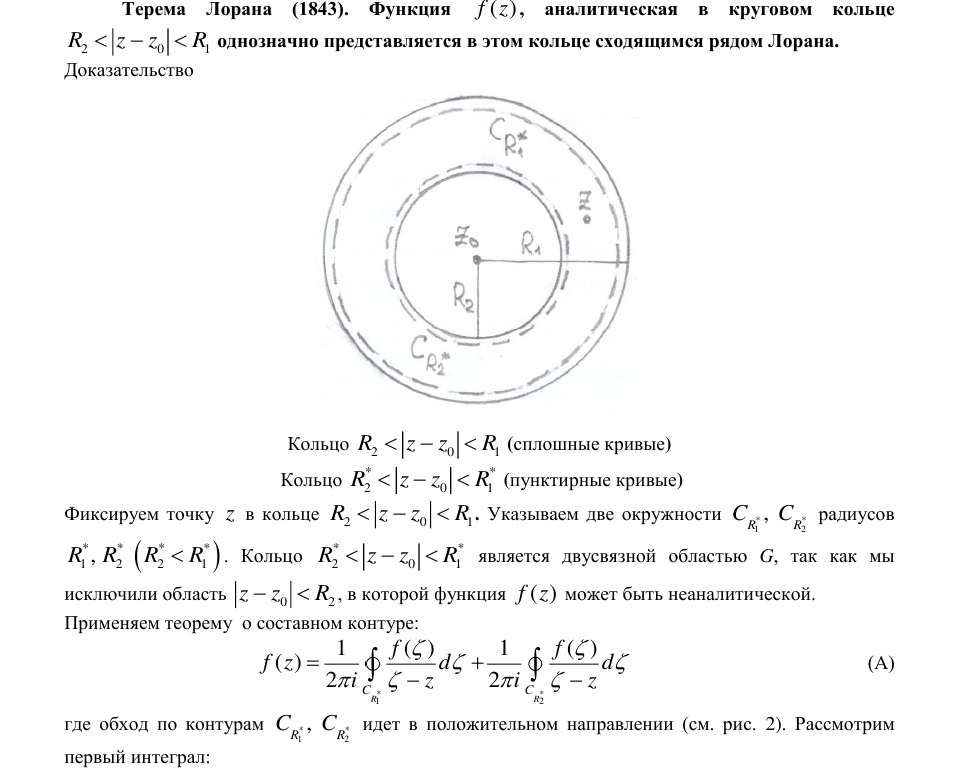
\includegraphics[width=\textwidth]{proof_loran_1}
\par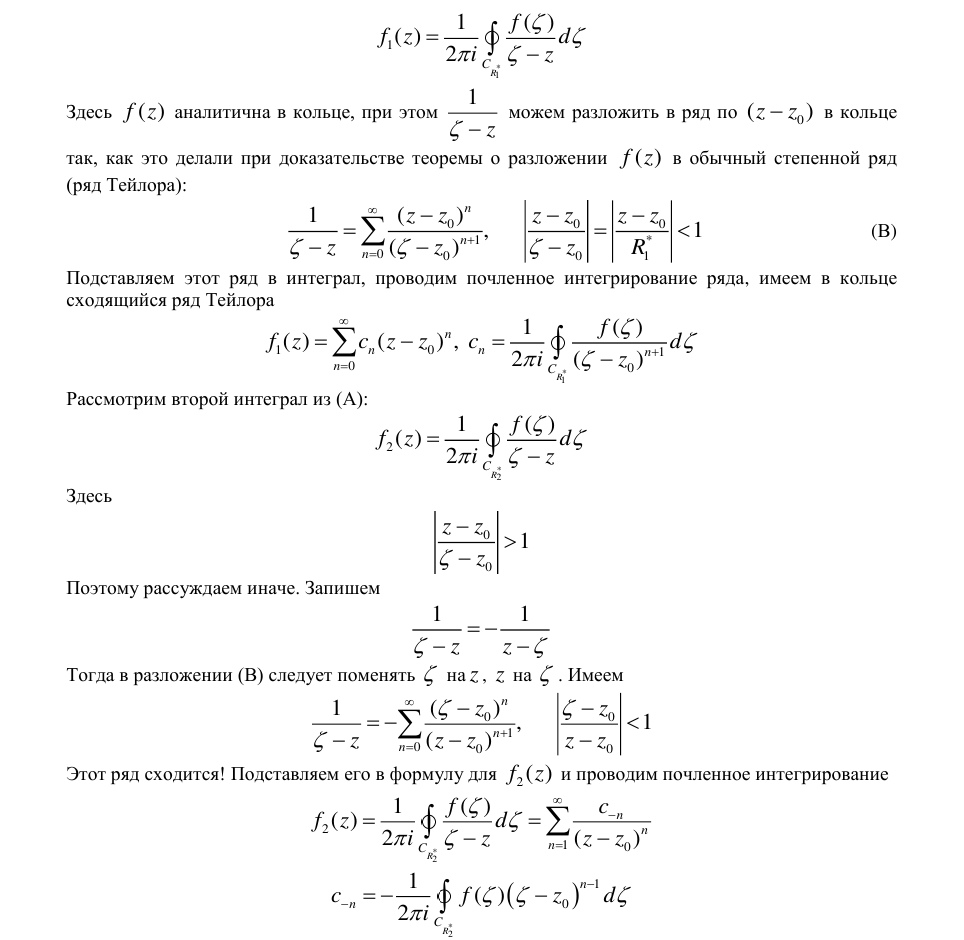
\includegraphics[width=\textwidth]{proof_loran_2}
\par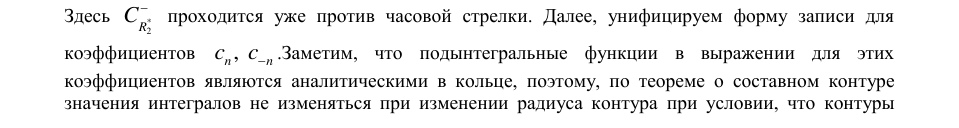
\includegraphics[width=\textwidth]{proof_loran_3}
\par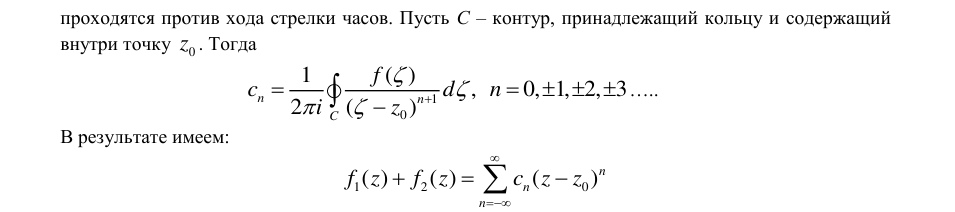
\includegraphics[width=\textwidth]{proof_loran_4}

\paragraph{Лорановское разложение функции $f(z)$ в окрестности бесконечно
удаленной точки}
\index{Лорановское разложение функции $f(z)$ в окрестности бесконечно
удаленной точки}
разложение $f(z)$ в ряд Лорана, сходящееся всюду вне круга
достаточно большого радиуса $R$ с центром в точке $z=0$


\section{Нули аналитических функций.}
\subsection{Понятие нуля аналитической функции}
Нулем функции порядка (кратности) $n$, называется точка $z_{0}$, если:
\begin{displaymath}
    f(z_{0})=0,\ \ f'(z_{0})=0,\ \ \ldots,
    \ \ f^{(n-1)}(z_{0})=0,\ \ f^{(n)}\neq 0
\end{displaymath}
\subsection{Теорема об изолированности нулей аналитических функций}
Пусть фукнция $f(z)$ аналитична в окрестности своего нуля $z_{0}$ и не
является тождественным нулем в этой крестности. Тогда $z_{0}$ является
изолированным нулем.
\par Доказательство: Так как $f(z)$ не равна тождественно нулю в
некоторой окрестности точки $z_{0}$, то ее можно представить в виде:
\begin{eqnarray*}
    f(z)=(z-z_{0})^{k}\varphi(z),
    \ \ \varphi(z_{0})\neq 0
\end{eqnarray*}
из аналитичности $\varphi(z)$ в точке $z_{0}$ следует ее непрерывность,
поэтому $\varphi(z_{0})\neq 0$ всюду в некоторой окрестности $z_{0}$,
поэтому нуль $z_{0}$ функции $f(z)$ изолирован.

\subsection{Теорема о тождественности аналитической фукнции $f(z)$ нулю
при наличии бесконечной последовательности ее нулей. Теорема о
единственности аналитических функций (без доказательств)}
\subsubsection{Теорема о тождественности аналитической фукнции $f(z)$ нулю
при наличии бесконечной последовательности ее нулей.}
Пусть функция $f(z)$ является аналитической в
области $G$ и обращается в ноль в различных точках бесконечной
последовательности $\{z_{n}\}$. Если последовательность $\{z_{n}\}$
сходится к точке $a$, принадлежащей области $G$, то $f(z)\equiv 0$ во
всей области $G$
\subsubsection{Теорема о единственности аналитических функций (без доказательств)}
Если функции $f_{1}(z),f_{2}(z)$, аналитические в областях $G_{1},G_{2}$
соответственно, имеющих общую область пересечения $G=G_{1}\cap G_{2}$,
совпадают в $G$, то существует единственная аналитическая функция такая,
что
\begin{eqnarray*}
    F(z)=\left\{\begin{aligned}
            f_{1}(z),\ \ z\in G_{1}\\
            f_{2}(z),\ \ z\in G_{2}
    \end{aligned} \right.
\end{eqnarray*}



\section{Изолированные особые точки ФКП.}
\paragraph{Особая точка.}\index{Особая точка} Точку $z_{0}$ функции
$f(z)$ будем называть особой, если в этой точке нарушается аналитичность
$f(z)$.
\paragraph{Изолированная особая точка $z_{0}$ функции $f(z)$}
\index{Изолированная особая точка}
Вокруг $z_{0}$ существует окрестность, в которой $f(z)$ аналитична
всюду, кроме самой точки $z_{0}$. Или формально: существует окрестность
$0<|z-z_{0}|<R_{1}$ этой точки, в кторой $f(z)$ аналитична.

\begin{enumerate}
    \item \index{Устранимая особая точка}
        \textit{Устранимая особая точка}:
        \subitem Существует предел $\lim\limits_{z\rightarrow
        z_{0}}f(z)=c_{0}$ (функцию можно доопределить)
        \subitem Ряд не содержит членов с отризацательными степенями
        разности $(z-z_{0})$
        \subitem \textbf{Теорема}. Если функция $f(z)$ аналитична в кольце
        $0<|z-z_{0}|<R_{1}$, ограничена в кольце, то $z_{0}$ есть
        устранимая особая точка
    \item Полюс функции :
        \subitem ряд Лорана содержит конечное число членов с
        отрицательными степенями разности $(z-z_{0})$
        \begin{eqnarray*}
            f(z)=\frac{c_{m}}{(z-z_{0})^{m}}
            +\ldots+
            \frac{c_{1}}{(z-z_{0})}
            +\sum\limits_{n=0}^{\infty}c_{n}(z-z_{0})^{n}
        \end{eqnarray*}
        \textit{полюс порядка $m$}
        \subitem Полюс порядка $n\ (n\geqslant 1)$ функции $f(z)$, если
        эта точка является нулем порядка $n$ для функции
        $\varphi=\frac{1}{f(z)}$. Если $n=1$ - полюс называют
        \textit{простым}
        \subitem При $z\to z_{0}$ модуль функции $f(z)$ неограниченно
        возрастает независимо от стремления $z$ к $z_{0}$
    \item Существенно особая точка 
        \subitem ряд Лорана содержит бесконечное
        число членов с отрицательными степенями разности $(z-z_{0})$
        \subitem Функция $f(z)$ в точке $z_{0}$ не имеет предела ни
        конечного, ни бесконечного
        \subitem \textbf{Теорема Сохоцкого-Казорати.}
        Если $z_{0}$ существенно особая точка функции $f(z)$, то для
        любого комплексного числа $A$ существует последовательность
        точек $z_{k}\to z_{0}$ така, что
        \begin{eqnarray*}
            \lim\limits_{k\rightarrow \infty}f(z_{k})=A
        \end{eqnarray*}
        \textit{частичные пределы этой функции не совпадают, принимают
        разные значения, предела в функции в точке $z_{0}$ не существует}
        \subitem $e^{\frac{1}{z}}$ - существенно особая точка.
        $\{z_{k}=\frac{1}{k}\},\ \{e^{k}\}\to \infty$,
        $\{z_{k}=-\frac{1}{k}\},\ \{e^{k}\}\to 0$,
        $A\neq 0,\ z_{k}=\frac{1}{\ln{A}+2k\pi i}$
\end{enumerate}
При рассмотрении характера точки, может быть подвох в том что
действительная часть стремится к нулю, а мнимая к бесконечности (или
наоборот). Такое бывает например в случае $z^{2}$

\par Утверждения:
\begin{enumerate}
    \itemsep0em
    \item $z_{0}$ - \textit{устранимая особая точка} ф-ции $f(z)$
        $\Leftrightarrow $ лораново разложения $f(z)$ в окрестности
        $z_{0}$ содержит только правильную часть
    \item $z_{0}$ - \textit{полюс функции} $f(z)$ $\Leftrightarrow $ главная
        часть лорановского разложения $f(z)$ в окрестности $z_{0}$
        содержит конечное число членов
    \item $z_{0}$ - \textit{существенно особая точка} для функции $f(z)$
        $\Leftrightarrow $ главная часть лорановского разложения в
        окрестности точки $z_{0}$ содержит бесконечно много членов
\end{enumerate}


\section{Применение вычетов к вычислению несобственных и контурных
интегралов.}
\nameref{основная теорема о вычетах}

\paragraph{Несобственные интегралы вида}
$\int\limits_{-\infty}^{\infty}f(x)\d{x}$
\begin{eqnarray*}
    \int\limits_{-\infty}^{\infty}f(x)\d{x}
    =2\pi i\sum\limits_{k=1}^{N}\res[f(z),z_{k}],\ \ x_{k}\textmd{
    особые точки функции $f(z)$ в верхней полуплоскости}
\end{eqnarray*}
\textbf{Лемма 1} Пусть функция $f(z)$ является
аналитической в верхней полуплоскости $\IM{z}>0$ всюду, за исключением
конечного числа изолированных особых точек, и существуют такие
положительные числа $R_{0},M$ и $\delta$, что для всех точек верхней
полуплоскости, удовлетворяющих условию $|z| > R_{0}$, имеет место
оценка:
\begin{eqnarray*}
    |f(z)|<\frac{M}{|z|^{1+\delta}},\ \ |z|>R_{0}
\end{eqnarray*}
Тогда
\begin{eqnarray*}
    \lim\limits_{R\rightarrow
    \infty}\int\limits_{C'_{R}}f(\zeta)\d{\zeta}
    =0
\end{eqnarray*}
где $C'_{R}$ представляет собой полуокружность $|z|=R$, $\IM{z}>0$
\par Доказательство леммы 1
\begin{eqnarray*}
    \left|\int\limits_{C'_{R}}f(\zeta)\d\zeta\right|
    \leqslant \int\limits_{C'_{R}}|f(\zeta)|\d{s}
    < \frac{M\pi R}{R^{1+\delta}}
    =\frac{\pi M}{R^{\delta}} \stackrel{R\to\infty}{\to} 0
\end{eqnarray*}
\par Доказательство основной теоремы: рассмотрим такой вот интеграл
\begin{eqnarray*}
    \int\limits_{-R}^{R}f(x)\d{x}+\int\limits_{C'_{R}}
    +\int\limits_{C'_{R}}f(z)\d{z}
    =2\pi i\sum\limits_{k=1}^{N}\res[f(z),z_{k}]
\end{eqnarray*}
т.к. выполнены условия леммы 1, то второе слагаемое при переходе
$R\to\infty$ равно нулю, правая (а следовательно и левая) от $R$ не
зависит, отсюда следует что теорема доказанна





\subsection{Интегралы от рациональных функций}
Пусть $f(x)=\frac{P_{m}(x)}{Q_{n}(x)}$ - рациональная функция, где
$P_{m}(x)$ и $Q_{n}(x)$ - многочлены соответственно степеней $m$ и $n$.
Условия:
\begin{enumerate}
    \itemsep0em
    \item $f(x)$ непрерывна на всей действительной оси ($Q_{n}(x)\neq 0$)
    \item $n \geqslant m+2$
\end{enumerate}
Можно применить формулу
\begin{displaymath}
    \int\limits_{-\infty}^{\infty}f(x)dx=2\pi i\sigma
\end{displaymath}
где $\sigma$ - сумма вычетов функции $f(z)$ во всех полюсах,
расположенных в верхней полуплоскости

\subsection{Вычисление интегралов содержащих правильную дробь умноженную
на синус или косинус}
\begin{displaymath}
    \int\limits_{0}^{\infty}R(x)\cos{\lambda x}dx
    ,\ \ \int\limits_{0}^{\infty}R(x)\sin{\lambda x}dx
\end{displaymath}
где $R(x)$ - правильная рациональная дробь, $\lambda > 0$ - любое
вещественное число
\par Поможет \textit{лемма Жордана}:
\par Пусть $g(z)$ - функция, аналитическая в верхней полуплоскости, за
исключением конечного числа особых точек, и стремится в этой
полуплоскости к нулю при $\left|z\right| \to \infty$. Тогда при
$\lambda>0$:
\begin{displaymath}
    \lim\limits_{R\rightarrow \infty}\int\limits_{C_{R}}g(z)e^{i\lambda
    z}=0
\end{displaymath}

\subsection{Вычисление интегралов, содержащих показательную функцию}
\begin{displaymath}
    \int\limits_{0}^{\infty}e^{-x^{2}}dx=\frac{\sqrt{\pi}}{2}
\end{displaymath}

\subsection{Вычисление интегралов содержащих рациональную функцию от
косинуса и синуса}
\begin{displaymath}
    \int\limits_{0}^{2\pi}R(\cos{x},\sin{x})dx
\end{displaymath}
где $R$ - рациональная функцию аргументов $\cos{x}$ и $\sin{x}$,
ограниченная внутри промежутка интегрирования
\par Полагаем, что $e^{ix}=z$, тогда $dx=\frac{dz}{iz}$ и
\begin{displaymath}
    \cos{x}=\frac{z^{2}+1}{2z}
    ,\ \ \sin{x}=\frac{z^{2}-1}{2iz}
\end{displaymath}
Интеграл принимает вид
\begin{displaymath}
    \int\limits_{C}F(z)dz
\end{displaymath}
где $C$ - окружность единичного радиуса с центром в начале координат.
Согласно теореме Коши о вычетах интеграл равен $2\pi\sigma i$, где
$\sigma$ - сумма вычетов относительно полюсов, заключенных внутри
окружности $C$

\subsubsection{Заменой}
Делаем замену $z=e^{ix}$. Тогда:
\begin{eqnarray*}
    dx&=&\frac{1}{i}\frac{dz}{z}
    ,\\ \cos{x}&=&\frac{1}{2}\left(e^{ix}+e^{-ix}\right)
=\frac{1}{2}\left(z+\frac{1}{z}\right)
    ,\\ \sin{x}&=&\frac{1}{2i}\left(e^{ix}-e^{-ix}\right)
=\frac{1}{2i}\left(z-\frac{1}{z}\right)
\end{eqnarray*}
Переменная $z$ пробегает окружность единичного радиуса
($\left|z\right|=1$). Интеграл приводится к интегралу по замкнутому
контуру:
\begin{eqnarray*}
I=\frac{1}{i}\int\limits_{\left|z\right|=1}
R\left(\frac{1}{2}\left(z+\frac{1}{z}\right),
\frac{1}{2i}\left(z-\frac{1}{z}\right)\right)
\frac{dz}{z}
\end{eqnarray*}

\section{Логарифмический вычет}
\subsection{Определение}
\paragraph{Логарифмическая производная функции $f(z)$}
\index{Логарифмическая производная функции}
производная от логарифма функции $f(z)$:
\begin{displaymath}
    \varphi(z)=\left[\ln f(z)\right]'=\frac{f'(z)}{f(z)}
\end{displaymath}
Вычет относительно точки, являющейся нулем функции $f(z)$, равен порядку
нуля, а относительно полюса функции - порядку этого полюса со знаком
минус
\par Пусть функция $f(z)\neq 0$аналитична во всех точках замкнутого
контура $C$. Величина
\begin{displaymath}
    \frac{1}{2\pi i}\int\limits_{C}\frac{f'(z)}{f(z)}dz
\end{displaymath}
называется логарифмическим вычетом функции $f(z)$ относительно
замкнутого контура $C$.
\subsection{Теорема о логарифмическом вычете}
Пусть функция $f(z)$ - аналитическая в замкнутой области $D$, кроме
конечного числа полюсов, и на границе $C$ этой области не умеет ни
нулей, ни полюсов. Тогда:
\begin{displaymath}
    \frac{1}{2\pi i}\int\limits_{C}\frac{f'(z)}{f(z)}dz=N-P
\end{displaymath}
где $N$ - число нулей $f(z)$ в $D$, $P$ - число полюсов $f(z)$ в $D$
\par Логарифмический вычет многочлена
\begin{displaymath}
    Q_{n}=\sum\limits_{k=0}^{n}a_{k}z^{k}
\end{displaymath}
относительно контура $C$ равен числу нулей этого многочлена (с учетом их
кратности) в области $D$, ограниченной контуром $C$

\subsection{Принцип аргумента}
Разность между количеством корней и полюсов с учетом их кратности
функции $f(z)$, заключающихся внутри замкнутой кривой $\Gamma$, равна
изменению $\Arg f(z)$ при обходе точкой $z$ контура $\Gamma$ в
положительном направлении, деленному на $2\pi$, т.е.:
\begin{eqnarray*}
    N-M=\frac{\Phi_{1}-\Phi_{0}}{2}
\end{eqnarray*}



\section{Преобразование Лапласа.}

\begin{eqnarray*}
w=az+b
\end{eqnarray*}

\begin{enumerate}
    \itemsep0em
    \item $b$ - сдвиг
    \item $a=w'_{z}$, $|a|$ - растяжение, $\Arg a$ - угол поворота
\end{enumerate}

\par Комфорное экспоненциальное:
Горизонтальные - в лучи (с углом наклона $C'$), вертикальные в круги (на
расстоянии $C$ переходят в окружность $e^{C}$)

\par Полоса (мн-во точек между двумя горизонтальными прямыми) -
бесконечная полоса. Ширина до $2\pi$


\section{Теоремы линейности и подобия преобразования Лапласа.}
\section{Основные теоремы операционного исчисления: дифференцирования
оригинала и изображения.}
\section{Основные теоремы операционного исчисления: запаздывания и
смещения.}
\section{Теорема обращения преобразования Лапласа.}
\section{Вывод основных соответствий между оригиналами и зображениями в
преобразовании Лапласа.}
\section{Решение линейных дифференциальных уравненийс постоянными
коэффициентами при помощи преобразования Лапласа.}
\section{Решение линейных систем дифференциальных уравнений.}
\section{Преобразование Лорана. Теорема опережения.}
\section{Вывод основных соответствий между оригиналами и зображениями
при преобразовании Лорана.}
\section{Преобразование Лорана. Теорема обращения и разложения.}
\section{Преобразование Лорана. Теорема дифференцирования изображения.}
\section{Преобразование Лорана. Умножение изображений. Теоремы о
предельных значениях.}
\section{Решение линейных разностных уравнений с помощью преобразования
Лорана.}
\section{Решение линейных разностных систем уравнений с помощью
преобразования Лорана}

\section{К экзамену}
\subsection{Формулировка теоремы об аналитичности степенного ряда в
круге сходимости}
Внутри круга сходимости степенной ряд сходится к аналитической функции.
Действительно, члены степенного ряда $u_{n}(z)=c_{n}(z-z_{0})^{n}$
представляют собой функции, аналитические на всей комплексной плоскости,
ряд сходится равномерно в любой замкнутой подобласти круга сходимости.
Следовательно, по первой теореме Вейерштрасса сумма ряда есть
аналитическая функция.
\subsection{Условия независимости интеграла от аналитической функции
$f(z)$ от вида кривой интегрирования $L$}
Возьмем замкнутый контур $L$ разобьем его на две части. По условию
аналитичности функции:
\begin{eqnarray*}
    \int\limits_{L}f(z)\d{z}=0
\end{eqnarray*}
разобьем этот контур пополам ($L_{1},L_{2}$). Получим
\begin{eqnarray*}
    &&\int\limits_{L_{1}}f(z)\d{z}+\int\limits_{L_{2}^{-}}f(z)\d{z}=0\\
    &&\int\limits_{L_{1}}f(z)\d{z}=\int\limits_{L_{2}}f(z)\d{z}
\end{eqnarray*}
отсюда следует, что интеграл не зависит от пути интегрирования

\subsection{Аналитическая функция $w=f(z)$ в точке $z_{0}$ как
конформное отображение окрестности $z_{0}$, основные свойства
конформного отображения}
\subsubsection{Аналитическая функция $w=f(z)$ в точке $z_{0}$ как
конформное отображение окрестности $z_{0}$}
\paragraph{Конформное отображения.}\index{Конформное отображение}
$f(z)$ обладает свойствами сохранения углов и постоянства растяжений.
Это значит что угол между любыми двумя гладкими кривыми, пересекающимися
в точке $z_{0}$, равен углу между их образами на плоскости $w$ в точке
$w_{0}=f(z_{0})$. Далее, бесконечно малые линейные элементы
преобразуются подобным образом с коэффициентом подобия $k=|f'(z_{0})|$.
\textit{Взаимно-однозначное отображение области $G$ комплексной
плоскости $z$ на область $D$ комплексной плоскости $w$ называется
конформным, если это отображение во всех точках $z\in G$ обладает
свойствами сохранения углоов и постоянства растяжений} (достаточно,
чтобы $f(z)$ была непрерывна)
\paragraph{Однолистное отображение.}\index{Однолистное отображение}
Отображение $F$ называют однолистным в области $G$, если в различных
точках этой области отображение $F$ принимает разные значения.
\par Однозначная аналитическая функция $f(z)$ в точке $z=z_{0}$ задает
конформное отображение малой окрестности точки $z_{0}$ на окрестность
точки $w_{0}=f(z_{0})$, если производная $f'(z_{0})$ существует и
$f'(z_{0})\neq 0$.

\subsubsection{Основные свойства конформного отображения}
\paragraph{Свойство 1.} $f'(z)\neq 0$ в каждой точке $z\in G$
\paragraph{Свойство 2.} Взаимно-однозначное отображение области $G$
комплексной плоскости $z$ на область $D$ комплексной плоскости $w$
является определяющим свойством конформного отображения

\subsection{Теорема о построении конформного отображения в области в
область через построение отображения границ (без доказательства)}
Пусть в конечной области $G$, ограниченной контуром $\gamma$ задана
однозначная функция $f(z)$, аналитическая в $\overline{G}$ и
отображающая контур $\gamma$ на некий контур $\Gamma$ комплексной
плоскости $w$ с сохранением направления обхода. Тогда функция $f(z)$
задает конформное отображение области $G$ на внутреннюю область $D$,
ограниченную контуром $\Gamma$

\subsection{Понятие аналитического продолжения аналитических функций}
Если функции $f_{1}(z), f_{2}(z)$, аналитические в областях
$G_{1},G_{2}$ соответственно, имеющих общую область пересечения
$G=G_{1}\cap G_{2}$, совпадают в $G$, то существует единственная
аналитическая функция такая, что
\begin{eqnarray*}
    F(z)=\left\{\begin{aligned}
            f_{1}(z),z\in G_{1}\\
            f_{2}(z),z\in G_{2}
    \end{aligned} \right.
\end{eqnarray*}
Здесь $f_{1}(z)$ является своим единственным аналитическим продолжением
с $G$ на $G_{1}$, $f_{2}(z)$ - единственное аналитическое продолжение с
$G$ на $G_{2}$.
\par Тогда функия $F(z)$ будет единственной аналитической функцией,
определенной в $G_{1}\cup G_{2}$, такой, что $F(z)$ совпадает с
$f_{1}(z)$ на $G_{1}$ и совпадает с $f_{2}(z)$ на $G_{2}$. Более того,
функция $f_{2}(z)$ является \textit{аналитическим продолжением функции}
$f_{1}(z)$ из области $G_{1}$ в область $G_{2}$, так как $f_{2}(z)$
"цепляет" $f_{1}(z)$ в области $G=G_{1}\cap G_{2}$. В отсутствии такой
"сцепки" $f_{2}(z)$ задается в области $G_{2}$ произвольно, таких
функций в области $G_{2}$ может быть бесконечно много, они не связаны
никак с $f_{1}(z)$. В этом случае говорить об аналитическом продолжении
$f_{1}(z)$ на область $G_{1}\cup G_{2}$ не приходится>
\par Область $G$ является "носителем" функции $f_{1}(z)$ на $G_{1}$ и,
она же, является носителем $f_{2}(z)$ на $G_{2}$. Поэтому $f_{2}(z)$ -
"клон" функции $f_{1}(z)$. Используя общепризнанный термин, $f_{2}(z)$ -
аналитическое продолжение $f_{1}(z)$

\subsection{Уравнение Лапласа, понятие гармонических функций. Теорема о
представлении вещественного решения уравнения Лапласа в виде сходящегося
степенного ряда}
\subsubsection{Уравнение Лапласа, понятие гармонических функций.}
\paragraph{Уравнение Лапласа} - линейное уравнение в частных производных
второго порядка:
\begin{eqnarray*}
\Delta u \triangleq
\frac{\partial^{2}u}{\partial x^{2}}
+\frac{\partial^{2}u}{\partial y^{2}}
+\frac{\partial^{2}u}{\partial z^{2}}=0
\end{eqnarray*}
Здесь $\Delta = \frac{\partial^{2}}{\partial
x^{2}}+\frac{\partial^{2}}{\partial y^{2}}
+\frac{\partial^{2}}{\partial z^{2}}$ - оператор Лапласа. Любое решение
$u(x,y,z)$ этого уравнения называют гармонической (в области
существования $D$) функцией. Это уравнение описывает многи процессы в
гидродинамике, теплопроводности, электростатики, гидравлики, в квантовой
механике, имеет большое значение в теории потенциала, в частности, в
теории гравитационного потенциала небесных тел.

\paragraph{Понятие гармонических функций}\index{Гармоническая функция} -
аналог понятия решения уравнения Лапласа (любое решение уравнения
Лапласа - гармоническая функция).

\subsubsection{Теорема о представлении вещественного решения уравнения Лапласа
в виде сходящегося степенного ряда}
Любое вещественное решение $u(x,y)$ уравнения лапласа является
аналитической функцией аргументов, т.е. в окрестности каждой точки
области $D$ она представима абсолютно сходящимся рядом
\begin{eqnarray*}
    u(x,y)=\sum\limits_{n=0}^{\infty}\sum\limits_{m=0}^{n}
    c_{nm}(x-x_{0})^{n-m}(y-y_{0})^{m}
\end{eqnarray*}
Доказательство: пользуясь следствием 1 (любое решение уравнения Лапласа
можно представить как действительную или мнимую части аналитической
функции $f(z)$) можно записать
\begin{eqnarray*}
    u(x,y)=\RE{f(z)}=\RE\left\{\sum\limits_{n=0}^{\infty}c_{n}(z-z_{0})^{n}\right\}
\end{eqnarray*}
Далее, записываем выражение для общего члена ряда функции $f(z)$:
\begin{eqnarray*}
    \RE\left\{c_{n}(z-z_{0})^{n}\right\}
    =\RE\left\{(\alpha_{n}+i\beta_{n})[(x-x_{0})+i(y-y_{0})]^{n}\right\}
    =\sum\limits_{m=0}^{n}c_{nm}(x-x_{0})^{n-m}(y-y_{0})^{m}
\end{eqnarray*}
(\textit{там получается биномиальное выражение})
После подстановки этого выражения в предыдущую формулу, докажем. Можно
показать, что радиус абсолютной сходимости этого ряда совпадает с
радиусом абсолютной сходимости ряда функции $f(z)$

\subsection{Постановка задачи о вычислении подъемной силы. Формула
Жуковского для вектора подъемной силы (без доказательств)}
\subsubsection{Постановка задачи о вычислении подъемной силы}
Подъемная сила, действующая на профиль крыла самолета, во время полета.
При скоростях, меньших скорости звука, воздух можно считать идеальной
несжимаемой жидкостью и пренебречь вихреобразованием вокруг крыла.
Считаем, что крыло имеет цилиндрическую форму с профилем, представленным
на рисунке (как капля). Полагаем, что для удобства изложения, что крыло
неподвижно и на него набегает поток с постоянной скоростью $V_{\infty}$,
равной скорости в бесконечности

\subsubsection{Формула Жуковского для вектора подъемной силы}
\begin{eqnarray*}
    F=-i\rho V_{\infty}\Gamma
\end{eqnarray*}
Сила $F$ является циркуляцией вектора $\Gamma$ вектора скорости вдоль
профиля $\gamma$, скоростью на бесконечности и эта сила перпендикулярна
направлению вектора скорости на бесконечности.
\subsubsection{Аналитическое продолжение}
Под аналитическим продолжением функции $f(z)$, определенной на некотором
множестве $G'$, подразумевается описание этой функции на возможно более
широкой области $G'\subset G$, в которой продолженная функция является
аналитической. Итак, $f(z)$ есть аналитическое продолжение с $G'$ в
область $G:G'\subset G$

\end{document}

